% Options for packages loaded elsewhere
\PassOptionsToPackage{unicode}{hyperref}
\PassOptionsToPackage{hyphens}{url}
\PassOptionsToPackage{dvipsnames,svgnames,x11names}{xcolor}
\documentclass[
  ignorenonframetext,
]{beamer}
\newif\ifbibliography
\usepackage{pgfpages}
\setbeamertemplate{caption}[numbered]
\setbeamertemplate{caption label separator}{: }
\setbeamercolor{caption name}{fg=normal text.fg}
\beamertemplatenavigationsymbolsempty
% remove section numbering
\setbeamertemplate{part page}{
  \centering
  \begin{beamercolorbox}[sep=16pt,center]{part title}
    \usebeamerfont{part title}\insertpart\par
  \end{beamercolorbox}
}
\setbeamertemplate{section page}{
  \centering
  \begin{beamercolorbox}[sep=12pt,center]{section title}
    \usebeamerfont{section title}\insertsection\par
  \end{beamercolorbox}
}
\setbeamertemplate{subsection page}{
  \centering
  \begin{beamercolorbox}[sep=8pt,center]{subsection title}
    \usebeamerfont{subsection title}\insertsubsection\par
  \end{beamercolorbox}
}
% Prevent slide breaks in the middle of a paragraph
\widowpenalties 1 10000
\raggedbottom
\AtBeginPart{
  \frame{\partpage}
}
\AtBeginSection{
  \ifbibliography
  \else
    \frame{\sectionpage}
  \fi
}
\AtBeginSubsection{
  \frame{\subsectionpage}
}
\usepackage{iftex}
\ifPDFTeX
  \usepackage[T1]{fontenc}
  \usepackage[utf8]{inputenc}
  \usepackage{textcomp} % provide euro and other symbols
\else % if luatex or xetex
  \usepackage{unicode-math} % this also loads fontspec
  \defaultfontfeatures{Scale=MatchLowercase}
  \defaultfontfeatures[\rmfamily]{Ligatures=TeX,Scale=1}
\fi
\usepackage{lmodern}
\usetheme[sectionpage=progressbar,numbering=fraction,progressbar=frametitle]{moloch}
\usefonttheme{serif} % use mainfont rather than sansfont for slide text
\ifPDFTeX\else
  % xetex/luatex font selection
  \setmainfont[]{Noto Sans}
  \setsansfont[]{Noto Sans}
  \setmonofont[]{Noto Sans Mono}
\fi
% Use upquote if available, for straight quotes in verbatim environments
\IfFileExists{upquote.sty}{\usepackage{upquote}}{}
\IfFileExists{microtype.sty}{% use microtype if available
  \usepackage[]{microtype}
  \UseMicrotypeSet[protrusion]{basicmath} % disable protrusion for tt fonts
}{}
\makeatletter
\@ifundefined{KOMAClassName}{% if non-KOMA class
  \IfFileExists{parskip.sty}{%
    \usepackage{parskip}
  }{% else
    \setlength{\parindent}{0pt}
    \setlength{\parskip}{6pt plus 2pt minus 1pt}}
}{% if KOMA class
  \KOMAoptions{parskip=half}}
\makeatother
\usepackage{color}
\usepackage{fancyvrb}
\newcommand{\VerbBar}{|}
\newcommand{\VERB}{\Verb[commandchars=\\\{\}]}
\DefineVerbatimEnvironment{Highlighting}{Verbatim}{commandchars=\\\{\}}
% Add ',fontsize=\small' for more characters per line
\newenvironment{Shaded}{}{}
\newcommand{\AlertTok}[1]{\textcolor[rgb]{1.00,0.00,0.00}{\textbf{#1}}}
\newcommand{\AnnotationTok}[1]{\textcolor[rgb]{0.38,0.63,0.69}{\textbf{\textit{#1}}}}
\newcommand{\AttributeTok}[1]{\textcolor[rgb]{0.49,0.56,0.16}{#1}}
\newcommand{\BaseNTok}[1]{\textcolor[rgb]{0.25,0.63,0.44}{#1}}
\newcommand{\BuiltInTok}[1]{\textcolor[rgb]{0.00,0.50,0.00}{#1}}
\newcommand{\CharTok}[1]{\textcolor[rgb]{0.25,0.44,0.63}{#1}}
\newcommand{\CommentTok}[1]{\textcolor[rgb]{0.38,0.63,0.69}{\textit{#1}}}
\newcommand{\CommentVarTok}[1]{\textcolor[rgb]{0.38,0.63,0.69}{\textbf{\textit{#1}}}}
\newcommand{\ConstantTok}[1]{\textcolor[rgb]{0.53,0.00,0.00}{#1}}
\newcommand{\ControlFlowTok}[1]{\textcolor[rgb]{0.00,0.44,0.13}{\textbf{#1}}}
\newcommand{\DataTypeTok}[1]{\textcolor[rgb]{0.56,0.13,0.00}{#1}}
\newcommand{\DecValTok}[1]{\textcolor[rgb]{0.25,0.63,0.44}{#1}}
\newcommand{\DocumentationTok}[1]{\textcolor[rgb]{0.73,0.13,0.13}{\textit{#1}}}
\newcommand{\ErrorTok}[1]{\textcolor[rgb]{1.00,0.00,0.00}{\textbf{#1}}}
\newcommand{\ExtensionTok}[1]{#1}
\newcommand{\FloatTok}[1]{\textcolor[rgb]{0.25,0.63,0.44}{#1}}
\newcommand{\FunctionTok}[1]{\textcolor[rgb]{0.02,0.16,0.49}{#1}}
\newcommand{\ImportTok}[1]{\textcolor[rgb]{0.00,0.50,0.00}{\textbf{#1}}}
\newcommand{\InformationTok}[1]{\textcolor[rgb]{0.38,0.63,0.69}{\textbf{\textit{#1}}}}
\newcommand{\KeywordTok}[1]{\textcolor[rgb]{0.00,0.44,0.13}{\textbf{#1}}}
\newcommand{\NormalTok}[1]{#1}
\newcommand{\OperatorTok}[1]{\textcolor[rgb]{0.40,0.40,0.40}{#1}}
\newcommand{\OtherTok}[1]{\textcolor[rgb]{0.00,0.44,0.13}{#1}}
\newcommand{\PreprocessorTok}[1]{\textcolor[rgb]{0.74,0.48,0.00}{#1}}
\newcommand{\RegionMarkerTok}[1]{#1}
\newcommand{\SpecialCharTok}[1]{\textcolor[rgb]{0.25,0.44,0.63}{#1}}
\newcommand{\SpecialStringTok}[1]{\textcolor[rgb]{0.73,0.40,0.53}{#1}}
\newcommand{\StringTok}[1]{\textcolor[rgb]{0.25,0.44,0.63}{#1}}
\newcommand{\VariableTok}[1]{\textcolor[rgb]{0.10,0.09,0.49}{#1}}
\newcommand{\VerbatimStringTok}[1]{\textcolor[rgb]{0.25,0.44,0.63}{#1}}
\newcommand{\WarningTok}[1]{\textcolor[rgb]{0.38,0.63,0.69}{\textbf{\textit{#1}}}}
\usepackage{longtable,booktabs,array}
\newcounter{none} % for unnumbered tables
\usepackage{calc} % for calculating minipage widths
\usepackage{caption}
% Make caption package work with longtable
\makeatletter
\def\fnum@table{\tablename~\thetable}
\makeatother
\setlength{\emergencystretch}{3em} % prevent overfull lines
\providecommand{\tightlist}{%
  \setlength{\itemsep}{0pt}\setlength{\parskip}{0pt}}
\usepackage{booktabs}
\usepackage{longtable}
\usepackage{colortbl}
\usepackage{etoolbox}
\usepackage{caption}
\usepackage{tikz}
\usetikzlibrary{arrows.meta, positioning, shapes.geometric, matrix}
\captionsetup[figure]{labelformat=empty}
\AtBeginEnvironment{longtable}{\scriptsize}
\AtBeginEnvironment{cslreferences}{\scriptsize}
\AtBeginEnvironment{Shaded}{\scriptsize}
\AtBeginEnvironment{verbatim}{\scriptsize}
\usepackage{bookmark}
\IfFileExists{xurl.sty}{\usepackage{xurl}}{} % add URL line breaks if available
\urlstyle{same}
\hypersetup{
  pdftitle={Bases de Dados Relacionais e SQL I},
  pdfauthor={Mário Antunes},
  colorlinks=true,
  linkcolor={Maroon},
  filecolor={Maroon},
  citecolor={Blue},
  urlcolor={Blue},
  pdfcreator={LaTeX via pandoc}}

\title{\texorpdfstring{Bases de Dados Relacionais e SQL
I}{Bases de Dados Relacionais e SQL I}}
\subtitle{\texorpdfstring{Laboratórios de Sistemas e
Serviços}{Laboratórios de Sistemas e Serviços}}
\author{\texorpdfstring{Mário Antunes}{Mário Antunes}}
\date{2026}
\institute{Universidade de Aveiro}

\begin{document}
\frame{\titlepage}

\section{Introdução}\label{introduuxe7uxe3o}

\begin{frame}{O que é uma Base de Dados?}
\protect\phantomsection\label{o-que-uxe9-uma-base-de-dados}
Um conjunto estruturado de dados mantido num computador, especialmente
um que seja acessível de várias formas.

\begin{itemize}
\tightlist
\item
  \textbf{Objetivo:} Armazenar, recuperar e gerir grandes quantidades de
  informação.
\item
  \textbf{Evolução:}

  \begin{itemize}
  \tightlist
  \item
    \textbf{Flat files:} CSV/Texto (Rápido mas limitado).
  \item
    \textbf{Hierárquico:} Estrutura em árvore (IBM IMS).
  \item
    \textbf{Relacional:} Tabelas com relações (O padrão desde os anos
    80).
  \item
    \textbf{NoSQL:} Esquemas flexíveis para big data (MongoDB, Redis).
  \end{itemize}
\end{itemize}
\end{frame}

\begin{frame}{O que é um RDBMS?}
\protect\phantomsection\label{o-que-uxe9-um-rdbms}
Um \textbf{Sistema de Gestão de Bases de Dados Relacionais (RDBMS)} é o
software que gere bases de dados relacionais.

\begin{itemize}
\tightlist
\item
  Fornece uma interface entre utilizadores/aplicações e os dados.
\item
  Exemplos: \textbf{SQLite, PostgreSQL, MySQL, Oracle, Microsoft SQL
  Server}.
\item
  Impõe o \textbf{Modelo Relacional} e a integridade dos dados.
\end{itemize}
\end{frame}

\begin{frame}{DB vs RDBMS}
\protect\phantomsection\label{db-vs-rdbms}
{\def\LTcaptype{none} % do not increment counter
\begin{longtable}[]{@{}
  >{\raggedright\arraybackslash}p{(\linewidth - 4\tabcolsep) * \real{0.3333}}
  >{\raggedright\arraybackslash}p{(\linewidth - 4\tabcolsep) * \real{0.3333}}
  >{\raggedright\arraybackslash}p{(\linewidth - 4\tabcolsep) * \real{0.3333}}@{}}
\toprule\noalign{}
\begin{minipage}[b]{\linewidth}\raggedright
Característica
\end{minipage} & \begin{minipage}[b]{\linewidth}\raggedright
Base de Dados (DB)
\end{minipage} & \begin{minipage}[b]{\linewidth}\raggedright
RDBMS
\end{minipage} \\
\midrule\noalign{}
\endhead
\textbf{Definição} & Uma coleção de dados. & Software para gerir
dados. \\
\textbf{Armazenamento} & Pode ser um simples ficheiro. & Organizado em
tabelas. \\
\textbf{Integridade} & Não é necessariamente imposta. & Impõe restrições
PK/FK. \\
\textbf{Acesso} & Acesso direto ao ficheiro. & Via SQL. \\
\textbf{Multutilizador} & Difícil de gerir. & Gere concorrência
(ACID). \\
\bottomrule\noalign{}
\end{longtable}
}
\end{frame}

\begin{frame}{Porquê não usar apenas Ficheiros? I}
\protect\phantomsection\label{porquuxea-nuxe3o-usar-apenas-ficheiros-i}
\begin{itemize}
\tightlist
\item
  \textbf{Redundância:} Os dados são frequentemente duplicados em vários
  ficheiros.
\item
  \textbf{Inconsistência:} Se alterar a morada de um utilizador num
  ficheiro, pode esquecer-se dos outros.
\item
  \textbf{Concorrência:} O que acontece se duas pessoas tentarem
  escrever no mesmo ficheiro ao mesmo tempo?
\item
  \textbf{Segurança:} Difícil de controlar quem vê cada parte dos dados.
\end{itemize}
\end{frame}

\begin{frame}[fragile]{Porquê não usar apenas Ficheiros? II}
\protect\phantomsection\label{porquuxea-nuxe3o-usar-apenas-ficheiros-ii}
\begin{itemize}
\tightlist
\item
  \textbf{Escalabilidade:} Pesquisar em 1 milhão de linhas num CSV é
  lento (\(O(N)\)).
\item
  \textbf{Relações:} Como ligar um aluno em \texttt{alunos.csv} a uma
  nota em \texttt{notas.csv} de forma eficiente?
\item
  \textbf{Integridade de Dados:} Como garantir que a ``Idade'' é sempre
  um número e não ``Vinte''?
\end{itemize}
\end{frame}

\section{O Modelo Relacional}\label{o-modelo-relacional}

\begin{frame}{Cenário Universitário}
\protect\phantomsection\label{cenuxe1rio-universituxe1rio}
Para compreender estes conceitos, utilizaremos o cenário de uma
\textbf{Base de Dados Universitária}:

\begin{itemize}
\tightlist
\item
  \textbf{University (Universidade):} A instituição de topo.
\item
  \textbf{Department (Departamento):} Ramos como ``Engenharia'' ou
  ``Artes''.
\item
  \textbf{Teacher (Professor):} Funcionários afetos aos departamentos.
\item
  \textbf{Course (Curso/Cadeira):} Disciplinas lecionadas por
  professores.
\item
  \textbf{Student (Aluno):} Indivíduos inscritos nos cursos.
\item
  \textbf{Enrollment (Inscrição):} A relação entre alunos e cursos.
\end{itemize}
\end{frame}

\begin{frame}{Diagrama Entidade-Relação (ER)}
\protect\phantomsection\label{diagrama-entidade-relauxe7uxe3o-er}
\begin{center}
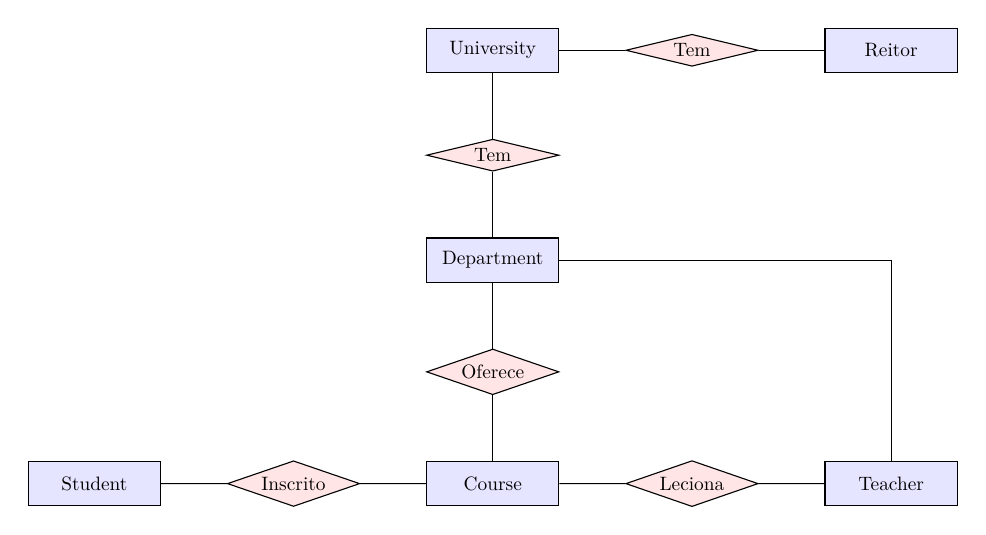
\begin{tikzpicture}[node distance=1.2cm, scale=0.7, every node/.style={transform shape}, 
    entity/.style={rectangle, draw, fill=blue!10, minimum width=2.4cm, minimum height=0.8cm},
    relationship/.style={diamond, draw, fill=red!10, aspect=2, inner sep=0pt, minimum width=2.4cm},
    attr/.style={ellipse, draw, fill=yellow!10, inner sep=1pt}]
    
    \node[entity] (univ) {University};
    \node[relationship, right=of univ] (has_r) {Tem};
    \node[entity, right=of has_r] (rect) {Reitor};
    \node[relationship, below=of univ] (has_d) {Tem};
    \node[entity, below=of has_d] (dept) {Department};
    \node[relationship, below=of dept] (offers) {Oferece};
    \node[entity, below=of offers] (course) {Course};
    \node[relationship, left=of course] (enrolled) {Inscrito};
    \node[entity, left=of enrolled] (stud) {Student};
    \node[relationship, right=of course] (teaches) {Leciona};
    \node[entity, right=of teaches] (teach) {Teacher};
    
    \draw (univ) -- (has_r);
    \draw (has_r) -- (rect);
    \draw (univ) -- (has_d);
    \draw (has_d) -- (dept);
    \draw (dept) -- (offers);
    \draw (offers) -- (course);
    \draw (course) -- (enrolled);
    \draw (enrolled) -- (stud);
    \draw (course) -- (teaches);
    \draw (teaches) -- (teach);
    \draw (teach) |- (dept);
\end{tikzpicture}
\end{center}
\end{frame}

\begin{frame}{Conceitos Base I}
\protect\phantomsection\label{conceitos-base-i}
Proposto por Edgar F. Codd in 1970, organiza os dados em uma ou mais
tabelas.

\begin{itemize}
\tightlist
\item
  \textbf{Tabela (Relação):} Uma coleção de elementos de dados
  organizados em linhas e colunas.
\item
  \textbf{Linha (Tuplo/Registo):} Representa um item único na tabela.
\item
  \textbf{Coluna (Atributo/Campo):} Representa uma propriedade
  específica dos itens.
\end{itemize}
\end{frame}

\begin{frame}{Conceitos Base II}
\protect\phantomsection\label{conceitos-base-ii}
\begin{center}
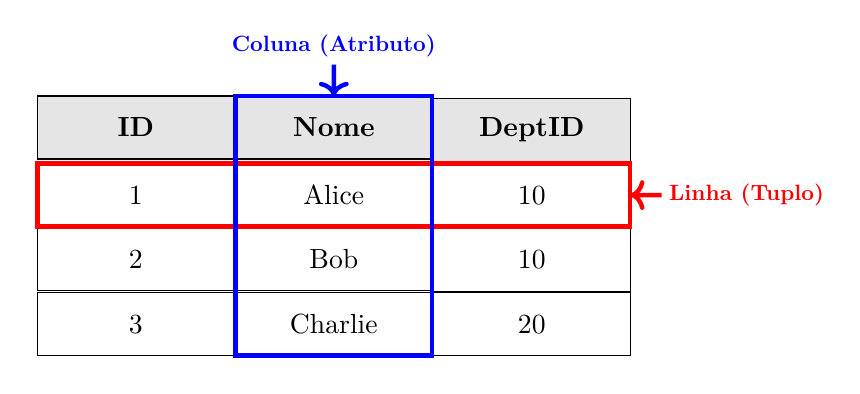
\begin{tikzpicture}[node distance=0cm, outer sep=0pt, scale=0.8, every node/.style={transform shape}]
    \tikzstyle{cell} = [rectangle, draw, minimum width=2.5cm, minimum height=0.8cm]
    \tikzstyle{header} = [cell, fill=gray!20, font=\bfseries]
    \matrix (m) [matrix of nodes, ampersand replacement=\&, nodes={cell}, row 1/.style={nodes={header}}] {
        ID \& Nome \& DeptID \\
        1 \& Alice \& 10 \\
        2 \& Bob \& 10 \\
        3 \& Charlie \& 20 \\
    };
    \draw[red, ultra thick] (m-2-1.north west) rectangle (m-2-3.south east);
    \node[right=0.5cm of m-2-3, red] (row) {\textbf{Linha (Tuplo)}};
    \draw[red, ultra thick, ->] (row) -- (m-2-3.east);
    \draw[blue, ultra thick] (m-1-2.north west) rectangle (m-4-2.south east);
    \node[above=0.5cm of m-1-2, blue] (col) {\textbf{Coluna (Atributo)}};
    \draw[blue, ultra thick, ->] (col) -- (m-1-2.north);
\end{tikzpicture}
\end{center}
\end{frame}

\begin{frame}[fragile]{Conceitos Base III: Chaves}
\protect\phantomsection\label{conceitos-base-iii-chaves}
\begin{itemize}
\tightlist
\item
  \textbf{Chave Primária (PK):} Um identificador único para cada linha.

  \begin{itemize}
  \tightlist
  \item
    \textbf{Chave Natural:} Algo que já existe (ex: NIF).
  \item
    \textbf{Chave Substituta:} Um ID artificial (ex:
    \texttt{id\ =\ 1,\ 2,\ 3}).
  \end{itemize}
\item
  \textbf{Chave Estrangeira (FK):} Uma coluna que cria uma ligação entre
  duas tabelas.
\item
  \textbf{Chave Composta:} Uma chave primária composta por duas ou mais
  colunas.
\end{itemize}
\end{frame}

\begin{frame}[fragile]{Integridade Referencial}
\protect\phantomsection\label{integridade-referencial}
Garante que as relações entre tabelas permanecem consistentes.

\begin{itemize}
\tightlist
\item
  Se \texttt{students.dept\_id} referencia \texttt{Department.id}, a
  base de dados impedirá:

  \begin{itemize}
  \tightlist
  \item
    Apagar um departamento que ainda tenha professores.
  \item
    Adicionar um professor a um departamento inexistente.
  \end{itemize}
\item
  \textbf{Ações:} \texttt{ON\ DELETE\ CASCADE} (apagar professores se o
  departamento for apagado) ou \texttt{ON\ DELETE\ SET\ NULL}.
\end{itemize}
\end{frame}

\begin{frame}[fragile]{Álgebra Relacional (Básicos)}
\protect\phantomsection\label{uxe1lgebra-relacional-buxe1sicos}
A base teórica do SQL.

\begin{itemize}
\tightlist
\item
  \textbf{Seleção (\(\sigma\)):} Filtrar linhas (SQL \texttt{WHERE}).
\item
  \textbf{Projeção (\(\pi\)):} Selecionar colunas (SQL
  \texttt{SELECT\ col1,\ col2}).
\item
  \textbf{Junção (\(\bowtie\)):} Combinar tabelas.
\item
  \textbf{União (\(\cup\)):} Combinar resultados de duas consultas.
\end{itemize}
\end{frame}

\begin{frame}{Normalização de Bases de Dados: Teoria 1NF}
\protect\phantomsection\label{normalizauxe7uxe3o-de-bases-de-dados-teoria-1nf}
O processo de organizar os dados para reduzir a redundância e melhorar a
integridade.

\begin{itemize}
\tightlist
\item
  \textbf{1NF (Primeira Forma Normal):}

  \begin{itemize}
  \tightlist
  \item
    Cada célula contém um único valor (atómico).
  \item
    Sem grupos repetidos de colunas.
  \item
    Cada linha é única (tem uma Chave Primária).
  \end{itemize}
\end{itemize}
\end{frame}

\begin{frame}{Normalização de Bases de Dados: Exemplo 1NF}
\protect\phantomsection\label{normalizauxe7uxe3o-de-bases-de-dados-exemplo-1nf}
\begin{center}
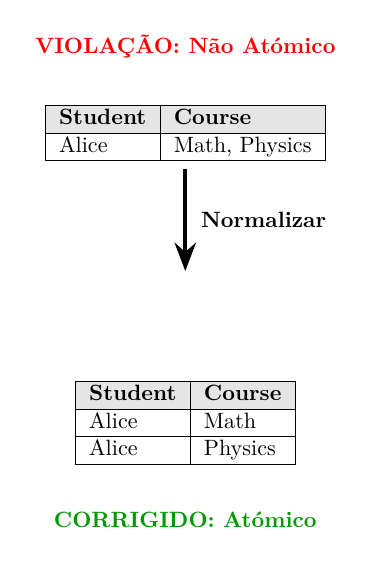
\begin{tikzpicture}[node distance=1.5cm, scale=0.8, every node/.style={transform shape}]
    % Violation
    \node (v1) {
    \begin{tabular}{|l|l|}
    \hline
    \rowcolor{gray!20} \textbf{Student} & \textbf{Course} \\ \hline
    Alice & Math, Physics \\ \hline
    \end{tabular}
    };
    \node[above=0.5cm of v1, red] {\textbf{VIOLAÇÃO: Não Atómico}};

    % Arrow
    \node[below=of v1] (arr) {};
    \draw[-{Stealth}, ultra thick] (v1.south) -- (arr.center) node[midway, right=3pt] {\textbf{Normalizar}};

    % Fixed
    \node[below=of arr] (f1) {
    \begin{tabular}{|l|l|}
    \hline
    \rowcolor{gray!20} \textbf{Student} & \textbf{Course} \\ \hline
    Alice & Math \\ \hline
    Alice & Physics \\ \hline
    \end{tabular}
    };
    \node[below=0.5cm of f1, green!60!black] {\textbf{CORRIGIDO: Atómico}};
\end{tikzpicture}
\end{center}
\end{frame}

\begin{frame}{Normalização de Bases de Dados: Teoria 2NF}
\protect\phantomsection\label{normalizauxe7uxe3o-de-bases-de-dados-teoria-2nf}
\begin{itemize}
\tightlist
\item
  \textbf{2NF (Segunda Forma Normal):}

  \begin{itemize}
  \tightlist
  \item
    Está na 1NF.
  \item
    Todos os atributos não-chave dependem totalmente de \emph{toda} a
    chave primária.
  \end{itemize}
\end{itemize}
\end{frame}

\begin{frame}{Normalização de Bases de Dados: Exemplo 2NF}
\protect\phantomsection\label{normalizauxe7uxe3o-de-bases-de-dados-exemplo-2nf}
\begin{center}
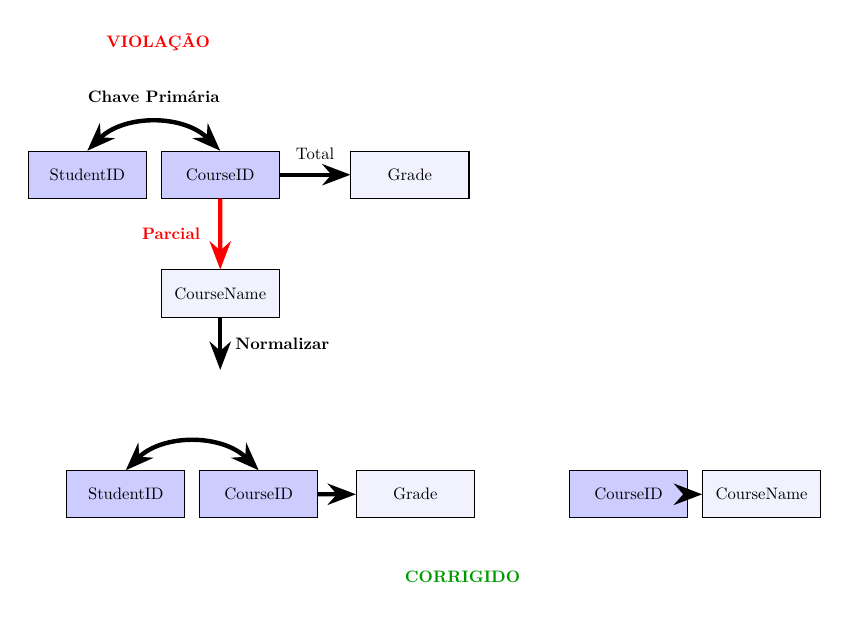
\begin{tikzpicture}[node distance=0.6cm, scale=0.6, every node/.style={transform shape}, box/.style={draw, rectangle, minimum width=2.5cm, minimum height=1cm, fill=blue!5}]
    % Violation
    \node[box, fill=blue!20] (sid) {StudentID};
    \node[box, fill=blue!20, right=0.3cm of sid] (cid) {CourseID};
    \node[box, right=1.5cm of cid] (grade) {Grade};
    \node[box, below=1.5cm of cid] (cname) {CourseName};
    \draw[{Stealth}-{Stealth}, ultra thick] (sid.north) to[bend left=45] node[midway, above=8pt] {\textbf{Chave Primária}} (cid.north);
    \draw[-{Stealth}, ultra thick] (cid.east) -- (grade.west) node[midway, above=5pt] {Total};
    \draw[-{Stealth}, ultra thick, red] (cid.south) -- (cname.north) node[midway, left=8pt] {\textbf{Parcial}};
    \node[above=2cm of sid, xshift=1.5cm, red] {\textbf{VIOLAÇÃO}};
    
    % Arrow
    \node[below=3.5cm of cid] (arr) {};
    \draw[-{Stealth}, ultra thick] (cname.south) -- (arr.center) node[midway, right=5pt] {\textbf{Normalizar}};

    % Fixed
    \node[box, fill=blue!20, below=2cm of arr, xshift=-2cm] (sid2) {StudentID};
    \node[box, fill=blue!20, right=0.3cm of sid2] (cid2) {CourseID};
    \node[box, right=0.8cm of cid2] (grade2) {Grade};
    
    \node[box, fill=blue!20, right=2cm of grade2] (cid3) {CourseID};
    \node[box, right=0.3cm of cid3] (cname2) {CourseName};
    
    \draw[{Stealth}-{Stealth}, ultra thick] (sid2.north) to[bend left=45] (cid2.north);
    \draw[-{Stealth}, ultra thick] (cid2.east) -- (grade2.west);
    \draw[-{Stealth}, ultra thick] (cid3.east) -- (cname2.west);
    \node[below=1cm of grade2, xshift=1cm, green!60!black] {\textbf{CORRIGIDO}};
\end{tikzpicture}
\end{center}
\end{frame}

\begin{frame}{Normalização de Bases de Dados: Teoria 3NF}
\protect\phantomsection\label{normalizauxe7uxe3o-de-bases-de-dados-teoria-3nf}
\begin{itemize}
\tightlist
\item
  \textbf{3NF (Terceira Forma Normal):}

  \begin{itemize}
  \tightlist
  \item
    Está na 2NF.
  \item
    Sem dependências transitivas (atributos não-chave não devem depender
    de outros atributos não-chave).
  \end{itemize}
\end{itemize}
\end{frame}

\begin{frame}{Normalização de Bases de Dados: Exemplo 3NF}
\protect\phantomsection\label{normalizauxe7uxe3o-de-bases-de-dados-exemplo-3nf}
\begin{center}
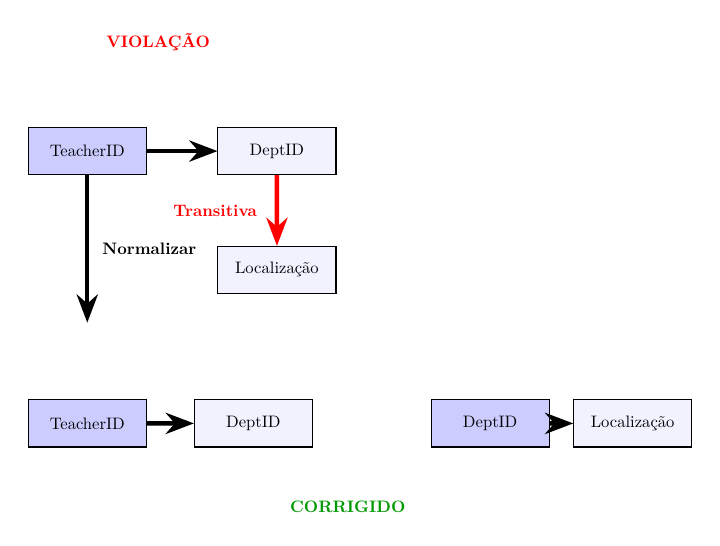
\begin{tikzpicture}[node distance=0.6cm, scale=0.6, every node/.style={transform shape}, box/.style={draw, rectangle, minimum width=2.5cm, minimum height=1cm, fill=blue!5}]
    % Violation
    \node[box, fill=blue!20] (tid) {TeacherID};
    \node[box, right=1.5cm of tid] (did) {DeptID};
    \node[box, below=1.5cm of did] (loc) {Localização};
    \draw[-{Stealth}, ultra thick] (tid) -- (did);
    \draw[-{Stealth}, ultra thick, red] (did) -- (loc) node[midway, left=8pt] {\textbf{Transitiva}};
    \node[above=1.5cm of tid, xshift=1.5cm, red] {\textbf{VIOLAÇÃO}};
    
    % Arrow
    \node[below=3cm of tid] (arr) {};
    \draw[-{Stealth}, ultra thick] (tid.south) -- (arr.center) node[midway, right=5pt] {\textbf{Normalizar}};

    % Fixed
    \node[box, fill=blue!20, below=1.5cm of arr] (tid2) {TeacherID};
    \node[box, right=1.0cm of tid2] (did2) {DeptID};
    
    \node[box, fill=blue!20, right=2.5cm of did2] (did3) {DeptID};
    \node[box, right=0.5cm of did3] (loc2) {Localização};
    
    \draw[-{Stealth}, ultra thick] (tid2) -- (did2);
    \draw[-{Stealth}, ultra thick] (did3) -- (loc2);
    \node[below=1cm of did2, xshift=2cm, green!60!black] {\textbf{CORRIGIDO}};
\end{tikzpicture}
\end{center}

\textbf{Objetivo:} ``The key, the whole key, and nothing but the key, so
help me Codd.''
\end{frame}

\begin{frame}{Relações em Bases de Dados I: 1:1}
\protect\phantomsection\label{relauxe7uxf5es-em-bases-de-dados-i-11}
\begin{itemize}
\tightlist
\item
  \textbf{Um-para-Um (1:1):} Uma entidade está relacionada com
  exatamente uma outra entidade.
\item
  Exemplo: Uma \textbf{University} tem um \textbf{Reitor}.
\end{itemize}

\begin{center}
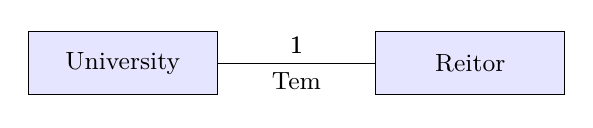
\begin{tikzpicture}[node distance=1.5cm, every node/.style={transform shape, font=\small}, 
    box/.style={rectangle, draw, fill=blue!10, minimum width=2.4cm, minimum height=0.8cm}]
    \node[box] (univ) {University};
    \node[box, right=2cm of univ] (rect) {Reitor};
    \draw (univ) -- node[above] {1} node[below] {Tem} (rect);
    \draw (rect) -- node[above] {1} (univ);
\end{tikzpicture}
\end{center}
\end{frame}

\begin{frame}{Relações em Bases de Dados II: 1:N}
\protect\phantomsection\label{relauxe7uxf5es-em-bases-de-dados-ii-1n}
\begin{itemize}
\tightlist
\item
  \textbf{Um-para-Muitos (1:N):} Uma entidade pode estar relacionada com
  muitas instâncias de outra.
\item
  Exemplo: Um \textbf{Department} tem muitos \textbf{Teachers}.
\end{itemize}

\begin{center}
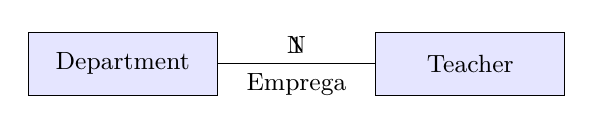
\begin{tikzpicture}[node distance=1.5cm, every node/.style={transform shape, font=\small}, 
    box/.style={rectangle, draw, fill=blue!10, minimum width=2.4cm, minimum height=0.8cm}]
    \node[box] (dept) {Department};
    \node[box, right=2cm of dept] (teach) {Teacher};
    \draw (dept) -- node[above] {1} node[below] {Emprega} (teach);
    \draw (teach) -- node[above] {N} (dept);
\end{tikzpicture}
\end{center}
\end{frame}

\begin{frame}{Relações em Bases de Dados III: N:M}
\protect\phantomsection\label{relauxe7uxf5es-em-bases-de-dados-iii-nm}
\begin{itemize}
\tightlist
\item
  \textbf{Muitos-para-Muitos (N:M):} Muitas instâncias de uma entidade
  relacionam-se com muitas de outra.
\item
  Exemplo: Muitos \textbf{Students} inscrevem-se em muitos
  \textbf{Courses}.
\item
  \textbf{Resolvido via Tabela de Junção.}
\end{itemize}

\begin{center}
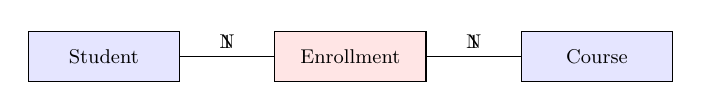
\begin{tikzpicture}[node distance=1.2cm, scale=0.8, every node/.style={transform shape, font=\small}, 
    box/.style={rectangle, draw, fill=blue!10, minimum width=2.4cm, minimum height=0.8cm}]
    \node[box] (stud) {Student};
    \node[box, right=1.5cm of stud, fill=red!10] (enroll) {Enrollment};
    \node[box, right=1.5cm of enroll] (course) {Course};
    \draw (stud) -- node[above] {1} (enroll);
    \draw (enroll) -- node[above] {N} (stud);
    \draw (course) -- node[above] {1} (enroll);
    \draw (enroll) -- node[above] {N} (course);
\end{tikzpicture}
\end{center}
\end{frame}

\section{Vantagens do RDBMS}\label{vantagens-do-rdbms}

\begin{frame}{Propriedades ACID I}
\protect\phantomsection\label{propriedades-acid-i}
Um RDBMS garante a integridade dos dados através do ACID:

\begin{itemize}
\tightlist
\item
  \textbf{Atomicidade:} ``Tudo ou nada.'' Se qualquer parte de uma
  transação falhar, toda a transação é revertida.
\item
  \textbf{Consistência:} A base de dados deve transitar de um estado
  válido para outro, seguindo todas as regras (restrições).
\end{itemize}
\end{frame}

\begin{frame}{Propriedades ACID II}
\protect\phantomsection\label{propriedades-acid-ii}
\begin{itemize}
\tightlist
\item
  \textbf{Isolamento:} Transações simultâneas não interferem; parecem
  correr sequencialmente.
\item
  \textbf{Durabilidade:} Uma vez confirmada (committed), os dados são
  permanentes, sobrevivendo a falhas do sistema.
\end{itemize}
\end{frame}

\section{SQL: Structured Query
Language}\label{sql-structured-query-language}

\begin{frame}{Diagrama do Esquema Relacional}
\protect\phantomsection\label{diagrama-do-esquema-relacional}
\begin{center}
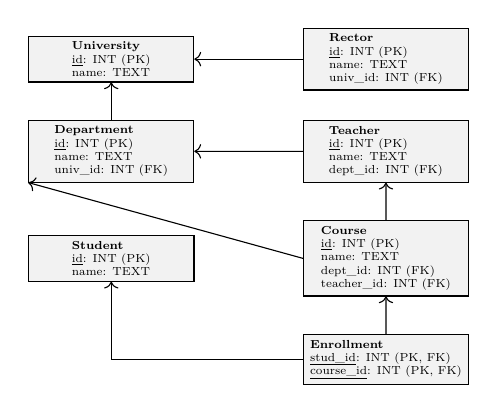
\begin{tikzpicture}[node distance=0.8cm, scale=0.6, every node/.style={transform shape, font=\scriptsize}, 
    table/.style={rectangle, draw, fill=gray!10, minimum width=3.5cm, align=left}]
    
    \node[table] (univ) {\textbf{University} \\ \underline{id}: INT (PK) \\ name: TEXT};
    \node[table, right=of univ, xshift=1.5cm] (rect) {\textbf{Rector} \\ \underline{id}: INT (PK) \\ name: TEXT \\ univ\_id: INT (FK)};
    \node[table, below=of univ] (dept) {\textbf{Department} \\ \underline{id}: INT (PK) \\ name: TEXT \\ univ\_id: INT (FK)};
    \node[table, right=of dept, xshift=1.5cm] (teach) {\textbf{Teacher} \\ \underline{id}: INT (PK) \\ name: TEXT \\ dept\_id: INT (FK)};
    \node[table, below=of teach] (course) {\textbf{Course} \\ \underline{id}: INT (PK) \\ name: TEXT \\ dept\_id: INT (FK) \\ teacher\_id: INT (FK)};
    \node[table, left=of course, xshift=-1.5cm] (stud) {\textbf{Student} \\ \underline{id}: INT (PK) \\ name: TEXT};
    \node[table, below=of course] (enroll) {\textbf{Enrollment} \\ \underline{stud\_id}: INT (PK, FK) \\ \underline{course\_id}: INT (PK, FK)};

    \draw[->] (rect.west) -- (univ.east);
    \draw[->] (dept.north) -- (univ.south);
    \draw[->] (teach.west) -- (dept.east);
    \draw[->] (course.north) -- (teach.south);
    \draw[->] (course.west) -- (dept.south west);
    \draw[->] (enroll.west) -| (stud.south);
    \draw[->] (enroll.north) -- (course.south);
\end{tikzpicture}
\end{center}
\end{frame}

\begin{frame}{O que é o SQL?}
\protect\phantomsection\label{o-que-uxe9-o-sql}
A linguagem padrão para lidar com Bases de Dados Relacionais.

\begin{itemize}
\tightlist
\item
  É uma linguagem \textbf{declarativa}: Diz à base de dados \emph{o que}
  quer, não \emph{como} obter.
\item
  \textbf{Padrão:} ANSI/ISO SQL, embora cada fornecedor adicione o seu
  próprio ``sabor''.
\end{itemize}
\end{frame}

\section{DDL: Data Definition
Language}\label{ddl-data-definition-language}

\begin{frame}[fragile]{Criar o Esquema I}
\protect\phantomsection\label{criar-o-esquema-i}
\begin{Shaded}
\begin{Highlighting}[]
\KeywordTok{CREATE} \KeywordTok{TABLE}\NormalTok{ University (}
    \KeywordTok{id} \DataTypeTok{INTEGER} \KeywordTok{PRIMARY} \KeywordTok{KEY}\NormalTok{ AUTOINCREMENT,}
\NormalTok{    name TEXT }\KeywordTok{NOT} \KeywordTok{NULL}
\NormalTok{);}

\KeywordTok{CREATE} \KeywordTok{TABLE}\NormalTok{ Rector (}
    \KeywordTok{id} \DataTypeTok{INTEGER} \KeywordTok{PRIMARY} \KeywordTok{KEY}\NormalTok{ AUTOINCREMENT,}
\NormalTok{    name TEXT }\KeywordTok{NOT} \KeywordTok{NULL}\NormalTok{,}
\NormalTok{    univ\_id }\DataTypeTok{INTEGER} \KeywordTok{UNIQUE}\NormalTok{,}
    \KeywordTok{FOREIGN} \KeywordTok{KEY}\NormalTok{ (univ\_id) }\KeywordTok{REFERENCES}\NormalTok{ University(}\KeywordTok{id}\NormalTok{)}
\NormalTok{);}
\end{Highlighting}
\end{Shaded}
\end{frame}

\begin{frame}[fragile]{Criar o Esquema II}
\protect\phantomsection\label{criar-o-esquema-ii}
\begin{Shaded}
\begin{Highlighting}[]
\KeywordTok{CREATE} \KeywordTok{TABLE}\NormalTok{ Department (}
    \KeywordTok{id} \DataTypeTok{INTEGER} \KeywordTok{PRIMARY} \KeywordTok{KEY}\NormalTok{ AUTOINCREMENT,}
\NormalTok{    name TEXT }\KeywordTok{NOT} \KeywordTok{NULL}\NormalTok{,}
\NormalTok{    univ\_id }\DataTypeTok{INTEGER}\NormalTok{,}
    \KeywordTok{FOREIGN} \KeywordTok{KEY}\NormalTok{ (univ\_id) }\KeywordTok{REFERENCES}\NormalTok{ University(}\KeywordTok{id}\NormalTok{)}
\NormalTok{);}

\KeywordTok{CREATE} \KeywordTok{TABLE}\NormalTok{ Teacher (}
    \KeywordTok{id} \DataTypeTok{INTEGER} \KeywordTok{PRIMARY} \KeywordTok{KEY}\NormalTok{ AUTOINCREMENT,}
\NormalTok{    name TEXT }\KeywordTok{NOT} \KeywordTok{NULL}\NormalTok{,}
\NormalTok{    dept\_id }\DataTypeTok{INTEGER}\NormalTok{,}
    \KeywordTok{FOREIGN} \KeywordTok{KEY}\NormalTok{ (dept\_id) }\KeywordTok{REFERENCES}\NormalTok{ Department(}\KeywordTok{id}\NormalTok{)}
\NormalTok{);}
\end{Highlighting}
\end{Shaded}
\end{frame}

\begin{frame}[fragile]{Criar o Esquema III}
\protect\phantomsection\label{criar-o-esquema-iii}
\begin{Shaded}
\begin{Highlighting}[]
\KeywordTok{CREATE} \KeywordTok{TABLE}\NormalTok{ Course (}
    \KeywordTok{id} \DataTypeTok{INTEGER} \KeywordTok{PRIMARY} \KeywordTok{KEY}\NormalTok{ AUTOINCREMENT,}
\NormalTok{    name TEXT }\KeywordTok{NOT} \KeywordTok{NULL}\NormalTok{,}
\NormalTok{    dept\_id }\DataTypeTok{INTEGER}\NormalTok{,}
\NormalTok{    teacher\_id }\DataTypeTok{INTEGER}\NormalTok{,}
    \KeywordTok{FOREIGN} \KeywordTok{KEY}\NormalTok{ (dept\_id) }\KeywordTok{REFERENCES}\NormalTok{ Department(}\KeywordTok{id}\NormalTok{),}
    \KeywordTok{FOREIGN} \KeywordTok{KEY}\NormalTok{ (teacher\_id) }\KeywordTok{REFERENCES}\NormalTok{ Teacher(}\KeywordTok{id}\NormalTok{)}
\NormalTok{);}

\KeywordTok{CREATE} \KeywordTok{TABLE}\NormalTok{ Student (}
    \KeywordTok{id} \DataTypeTok{INTEGER} \KeywordTok{PRIMARY} \KeywordTok{KEY}\NormalTok{ AUTOINCREMENT,}
\NormalTok{    name TEXT }\KeywordTok{NOT} \KeywordTok{NULL}
\NormalTok{);}
\end{Highlighting}
\end{Shaded}
\end{frame}

\begin{frame}[fragile]{Criar o Esquema IV}
\protect\phantomsection\label{criar-o-esquema-iv}
\begin{Shaded}
\begin{Highlighting}[]
\KeywordTok{CREATE} \KeywordTok{TABLE}\NormalTok{ Enrollment (}
\NormalTok{    stud\_id }\DataTypeTok{INTEGER}\NormalTok{,}
\NormalTok{    course\_id }\DataTypeTok{INTEGER}\NormalTok{,}
    \KeywordTok{PRIMARY} \KeywordTok{KEY}\NormalTok{ (stud\_id, course\_id),}
    \KeywordTok{FOREIGN} \KeywordTok{KEY}\NormalTok{ (stud\_id) }\KeywordTok{REFERENCES}\NormalTok{ Student(}\KeywordTok{id}\NormalTok{),}
    \KeywordTok{FOREIGN} \KeywordTok{KEY}\NormalTok{ (course\_id) }\KeywordTok{REFERENCES}\NormalTok{ Course(}\KeywordTok{id}\NormalTok{)}
\NormalTok{);}
\end{Highlighting}
\end{Shaded}
\end{frame}

\section{DML: Data Manipulation
Language}\label{dml-data-manipulation-language}

\begin{frame}[fragile]{Inserir Dados I}
\protect\phantomsection\label{inserir-dados-i}
\begin{Shaded}
\begin{Highlighting}[]
\KeywordTok{INSERT} \KeywordTok{INTO}\NormalTok{ University (name) }\KeywordTok{VALUES}\NormalTok{ (}\StringTok{\textquotesingle{}Univ. Aveiro\textquotesingle{}}\NormalTok{);}

\KeywordTok{INSERT} \KeywordTok{INTO}\NormalTok{ Rector (name, univ\_id) }\KeywordTok{VALUES}\NormalTok{ (}\StringTok{\textquotesingle{}Prof. Paulo Jorge Ferreira\textquotesingle{}}\NormalTok{, }\DecValTok{1}\NormalTok{);}

\KeywordTok{INSERT} \KeywordTok{INTO}\NormalTok{ Department (name, univ\_id) }\KeywordTok{VALUES}\NormalTok{ (}\StringTok{\textquotesingle{}DETI\textquotesingle{}}\NormalTok{, }\DecValTok{1}\NormalTok{), (}\StringTok{\textquotesingle{}DMat\textquotesingle{}}\NormalTok{, }\DecValTok{1}\NormalTok{);}

\KeywordTok{INSERT} \KeywordTok{INTO}\NormalTok{ Teacher (name, dept\_id) }\KeywordTok{VALUES}\NormalTok{ (}\StringTok{\textquotesingle{}Dr. Smith\textquotesingle{}}\NormalTok{, }\DecValTok{1}\NormalTok{), (}\StringTok{\textquotesingle{}Dr. Taylor\textquotesingle{}}\NormalTok{, }\DecValTok{2}\NormalTok{);}
\end{Highlighting}
\end{Shaded}
\end{frame}

\begin{frame}[fragile]{Inserir Dados II}
\protect\phantomsection\label{inserir-dados-ii}
\begin{Shaded}
\begin{Highlighting}[]
\KeywordTok{INSERT} \KeywordTok{INTO}\NormalTok{ Course (name, dept\_id, teacher\_id) }
\KeywordTok{VALUES}\NormalTok{ (}\StringTok{\textquotesingle{}Relational Databases\textquotesingle{}}\NormalTok{, }\DecValTok{1}\NormalTok{, }\DecValTok{1}\NormalTok{), (}\StringTok{\textquotesingle{}Linear Algebra\textquotesingle{}}\NormalTok{, }\DecValTok{2}\NormalTok{, }\DecValTok{2}\NormalTok{);}

\KeywordTok{INSERT} \KeywordTok{INTO}\NormalTok{ Student (name) }\KeywordTok{VALUES}\NormalTok{ (}\StringTok{\textquotesingle{}Alice\textquotesingle{}}\NormalTok{), (}\StringTok{\textquotesingle{}Bob\textquotesingle{}}\NormalTok{);}

\KeywordTok{INSERT} \KeywordTok{INTO}\NormalTok{ Enrollment (stud\_id, course\_id) }
\KeywordTok{VALUES}\NormalTok{ (}\DecValTok{1}\NormalTok{, }\DecValTok{1}\NormalTok{), (}\DecValTok{1}\NormalTok{, }\DecValTok{2}\NormalTok{), (}\DecValTok{2}\NormalTok{, }\DecValTok{1}\NormalTok{);}
\end{Highlighting}
\end{Shaded}
\end{frame}

\section{DQL: Consultas Complexas}\label{dql-consultas-complexas}

\begin{frame}[fragile]{Exemplo de Consulta Complexa}
\protect\phantomsection\label{exemplo-de-consulta-complexa}
\begin{Shaded}
\begin{Highlighting}[]
\KeywordTok{SELECT}\NormalTok{ s.name }\KeywordTok{AS}\NormalTok{ Aluno, c.name }\KeywordTok{AS}\NormalTok{ Cadeira, t.name }\KeywordTok{AS}\NormalTok{ Professor, }
\NormalTok{       d.name }\KeywordTok{AS}\NormalTok{ Dept, u.name }\KeywordTok{AS}\NormalTok{ Univ, r.name }\KeywordTok{AS}\NormalTok{ Reitor}
\KeywordTok{FROM}\NormalTok{ Student s}
\KeywordTok{JOIN}\NormalTok{ Enrollment e }\KeywordTok{ON}\NormalTok{ s.}\KeywordTok{id} \OperatorTok{=}\NormalTok{ e.stud\_id}
\KeywordTok{JOIN}\NormalTok{ Course c }\KeywordTok{ON}\NormalTok{ e.course\_id }\OperatorTok{=}\NormalTok{ c.}\KeywordTok{id}
\KeywordTok{JOIN}\NormalTok{ Teacher t }\KeywordTok{ON}\NormalTok{ c.teacher\_id }\OperatorTok{=}\NormalTok{ t.}\KeywordTok{id}
\KeywordTok{JOIN}\NormalTok{ Department d }\KeywordTok{ON}\NormalTok{ t.dept\_id }\OperatorTok{=}\NormalTok{ d.}\KeywordTok{id}
\KeywordTok{JOIN}\NormalTok{ University u }\KeywordTok{ON}\NormalTok{ d.univ\_id }\OperatorTok{=}\NormalTok{ u.}\KeywordTok{id}
\KeywordTok{JOIN}\NormalTok{ Rector r }\KeywordTok{ON}\NormalTok{ u.}\KeywordTok{id} \OperatorTok{=}\NormalTok{ r.univ\_id}
\KeywordTok{ORDER} \KeywordTok{BY}\NormalTok{ s.name }\KeywordTok{ASC}\NormalTok{;}
\end{Highlighting}
\end{Shaded}
\end{frame}

\begin{frame}{Resultados Esperados I}
\protect\phantomsection\label{resultados-esperados-i}
{\def\LTcaptype{none} % do not increment counter
\begin{longtable}[]{@{}lll@{}}
\toprule\noalign{}
Aluno & Cadeira & Professor \\
\midrule\noalign{}
\endhead
Alice & Relational Databases & Dr.~Smith \\
Alice & Linear Algebra & Dr.~Taylor \\
Bob & Relational Databases & Dr.~Smith \\
\bottomrule\noalign{}
\end{longtable}
}
\end{frame}

\begin{frame}{Resultados Esperados II}
\protect\phantomsection\label{resultados-esperados-ii}
{\def\LTcaptype{none} % do not increment counter
\begin{longtable}[]{@{}lll@{}}
\toprule\noalign{}
Dept & Univ & Reitor \\
\midrule\noalign{}
\endhead
DETI & Univ. Aveiro & Prof.~Paulo Jorge\ldots{} \\
DMat & Univ. Aveiro & Prof.~Paulo Jorge\ldots{} \\
DETI & Univ. Aveiro & Prof.~Paulo Jorge\ldots{} \\
\bottomrule\noalign{}
\end{longtable}
}
\end{frame}

\section{Sumário}\label{sumuxe1rio}

\begin{frame}{Sumário}
\protect\phantomsection\label{sumuxe1rio-1}
\begin{itemize}
\tightlist
\item
  \textbf{RDBMS:} Software que impõe o modelo relacional (SQLite,
  MySQL).
\item
  \textbf{ACID:} Garante fiabilidade (Atomicidade, Consistência,
  Isolamento, Durabilidade).
\item
  \textbf{Cardinalidade:} Visualizada via diagramas 1:1, 1:N e N:M.
\item
  \textbf{SQL:} DDL (Esquema), DML (Dados) e DQL (Consultas)
  abrangentes.
\end{itemize}
\end{frame}

\end{document}
